\chapter{Results and Evaluation}
\label{ch:results}

This chapter answers RQ1 and RQ2 using the attacker model and the exact evaluation of
Chapter~\ref{ch:formulation}. Every number in it is reproduced, with fixed seeds, by the
command \code{python -m simulator.experiments}, which takes about one minute on eight cores.

\section{Experimental Protocol}

\begin{itemize}
  \item \textbf{Policies:} Q-learning and SARSA on the 30-state observation; an $\varepsilon$-greedy
    bandit that ignores the state; the static honeypot (always \act{allow}); a uniformly random policy.
  \item \textbf{Hyper-parameters:} $\gamma = 0.9$; $\varepsilon$ from 0.3 decaying by a factor
    of 0.995 per episode to a floor of 0.05; $\alpha_n = n^{-0.7}$ per state--action pair.
  \item \textbf{Main experiment:} balanced population, 20 seeds $\times$ 20{,}000 episodes per
    learner. At the end, each run's greedy policy is evaluated \emph{exactly}. The spread across
    seeds therefore reflects learning alone, not evaluation noise.
  \item \textbf{Statistics:} 95\% Student-$t$ confidence intervals over seeds; a one-sided
    one-sample $t$-test of Q-learning against the deterministic static value; Welch's $t$-test
    between Q-learning and SARSA.
  \item \textbf{Seed hygiene:} the step-size schedule was chosen in a pilot on disjoint seeds
    and fixed before the reported runs. Main, sensitivity, ablation and diagnostic runs all use
    disjoint seed ranges.
\end{itemize}

\paragraph{Validation of the exact evaluator.} For the policy learned by seed~0, 50{,}000
simulated episodes give a mean return of $5.442 \pm 0.043$ and $3.884 \pm 0.027$ commands. The
exact values are $5.464$ and $3.899$, both inside the intervals. The unit tests check the same
agreement for three further policies.

\section{RQ1: Learned versus Static Responses}

\begin{table}[H]
\centering
\begin{tabular}{@{}lccc@{}}
\toprule
\textbf{Policy} & \textbf{Return} & \textbf{Commands/session} & \textbf{Intel/session} \\
\midrule
Q-learning & $\mathbf{5.686 \pm 0.051}$ & $4.056 \pm 0.034$ & $9.91 \pm 0.10$ \\
SARSA & $\mathbf{5.702 \pm 0.026}$ & $4.064 \pm 0.018$ & $9.93 \pm 0.05$ \\
$\varepsilon$-greedy bandit & $5.503 \pm 0.021$ & $3.982 \pm 0.028$ & $9.58 \pm 0.03$ \\
Static (always \act{allow}) & $5.542$ & $4.034$ & $9.64$ \\
Random & $1.949$ & $2.015$ & $3.91$ \\
\midrule
Best observable policy & $5.783$ & $4.157$ & $10.22$ \\
Oracle (type observed) & $5.935$ & -- & -- \\
\bottomrule
\end{tabular}
\caption{Exact expected performance of the final greedy policies (mean $\pm$ 95\% CI over 20 seeds).}
\label{tab:main}
\end{table}

\begin{figure}[H]
\centering
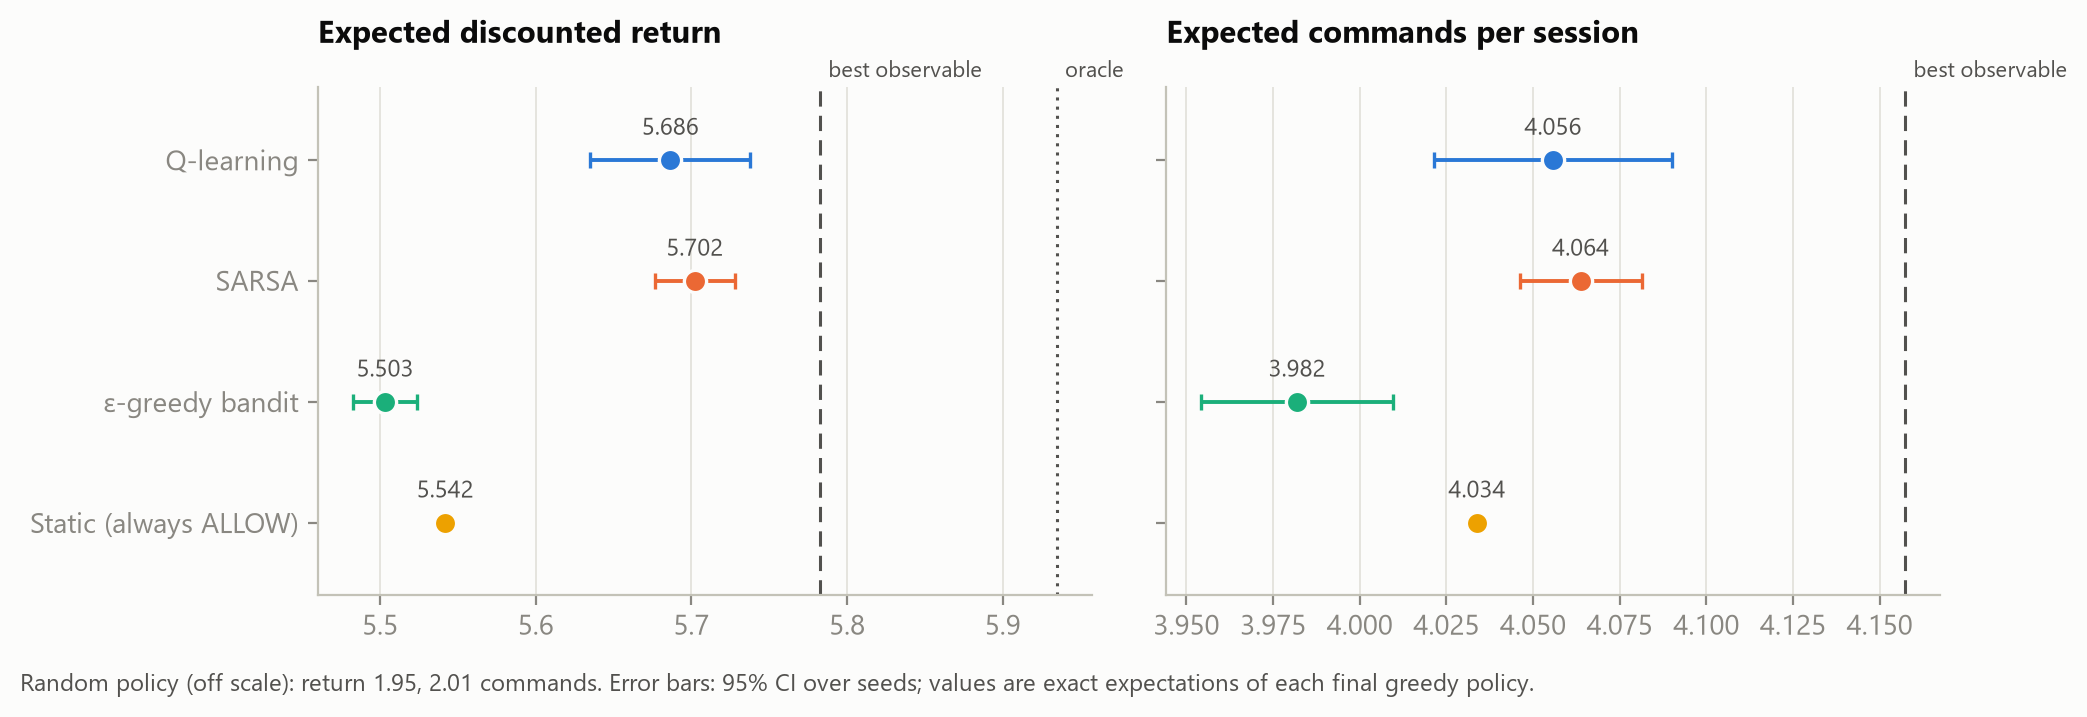
\includegraphics[width=\textwidth]{fig_final_performance.png}
\caption{Final greedy policies against the best observable policy and the oracle.}
\label{fig:final}
\end{figure}

\begin{enumerate}
  \item \textbf{Learning beats the static honeypot.} Q-learning's return exceeds static by
    2.6\% ($t = 5.88$, $p = 5.8 \times 10^{-6}$, $n = 20$). It recovers $60\% \pm 21\%$ of the
    gap between static and the best observable policy. Engagement rises by 0.5\% and captured
    intelligence by 2.8\%: the gain comes from \emph{which} sessions are prolonged, namely
    credential-hunting ones, more than from how many commands are seen.
  \item \textbf{Q-learning and SARSA are indistinguishable} (Welch $p = 0.57$).
  \item \textbf{State matters.} The bandit, which must pick one action for all situations,
    does \emph{worse} than static. No single action beats \act{allow} everywhere.
  \item \textbf{The remaining headroom needs information the honeypot lacks.} The oracle exceeds
    the best observable policy by a further 2.6\%, but only by knowing the attacker's type.
\end{enumerate}

\subsection{What the Agent Learns}

The best observable policy departs from \act{allow} in exactly one place: \textbf{\act{fake} on
credential access, in every phase}. Figure~\ref{fig:policymap} shows that Q-learning finds this
in every seed for the early and mid phases and in 80\% of seeds for the late phase. The policy
agrees with the best one in 68\% of states, yet achieves 60\% of its gain. Most disagreements
occur where actions are nearly equivalent (bots barely react) or in rarely visited states,
where a wrong choice costs almost nothing.

\begin{figure}[H]
\centering
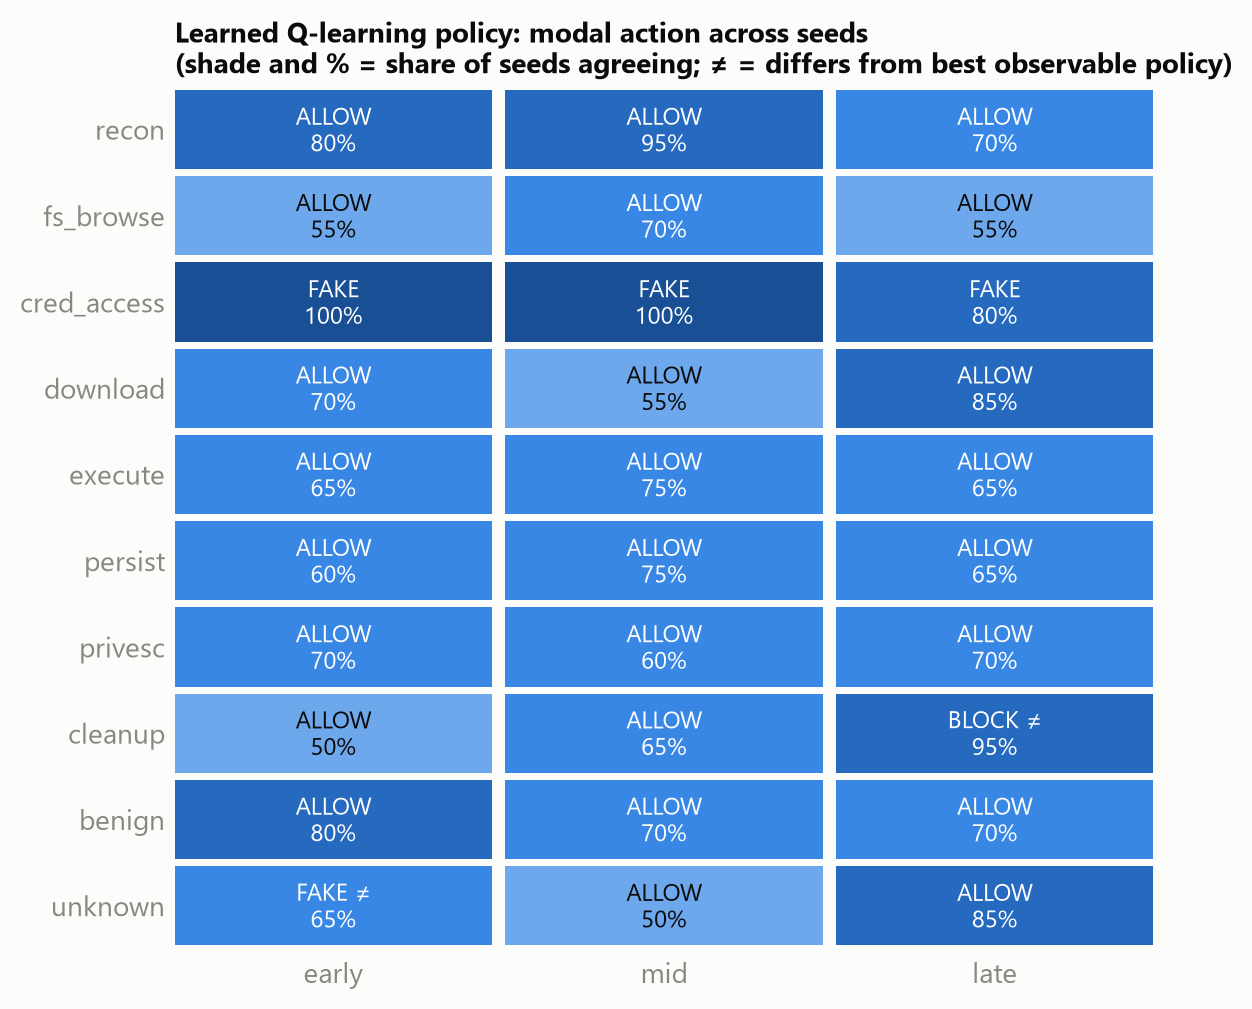
\includegraphics[width=0.78\textwidth]{fig_policy_map.png}
\caption{Modal action learned by Q-learning in each state across 20 seeds; the shading gives the share of seeds that agree.}
\label{fig:policymap}
\end{figure}

\subsection{Learning Dynamics and the Cost of Exploration}

\begin{figure}[H]
\centering
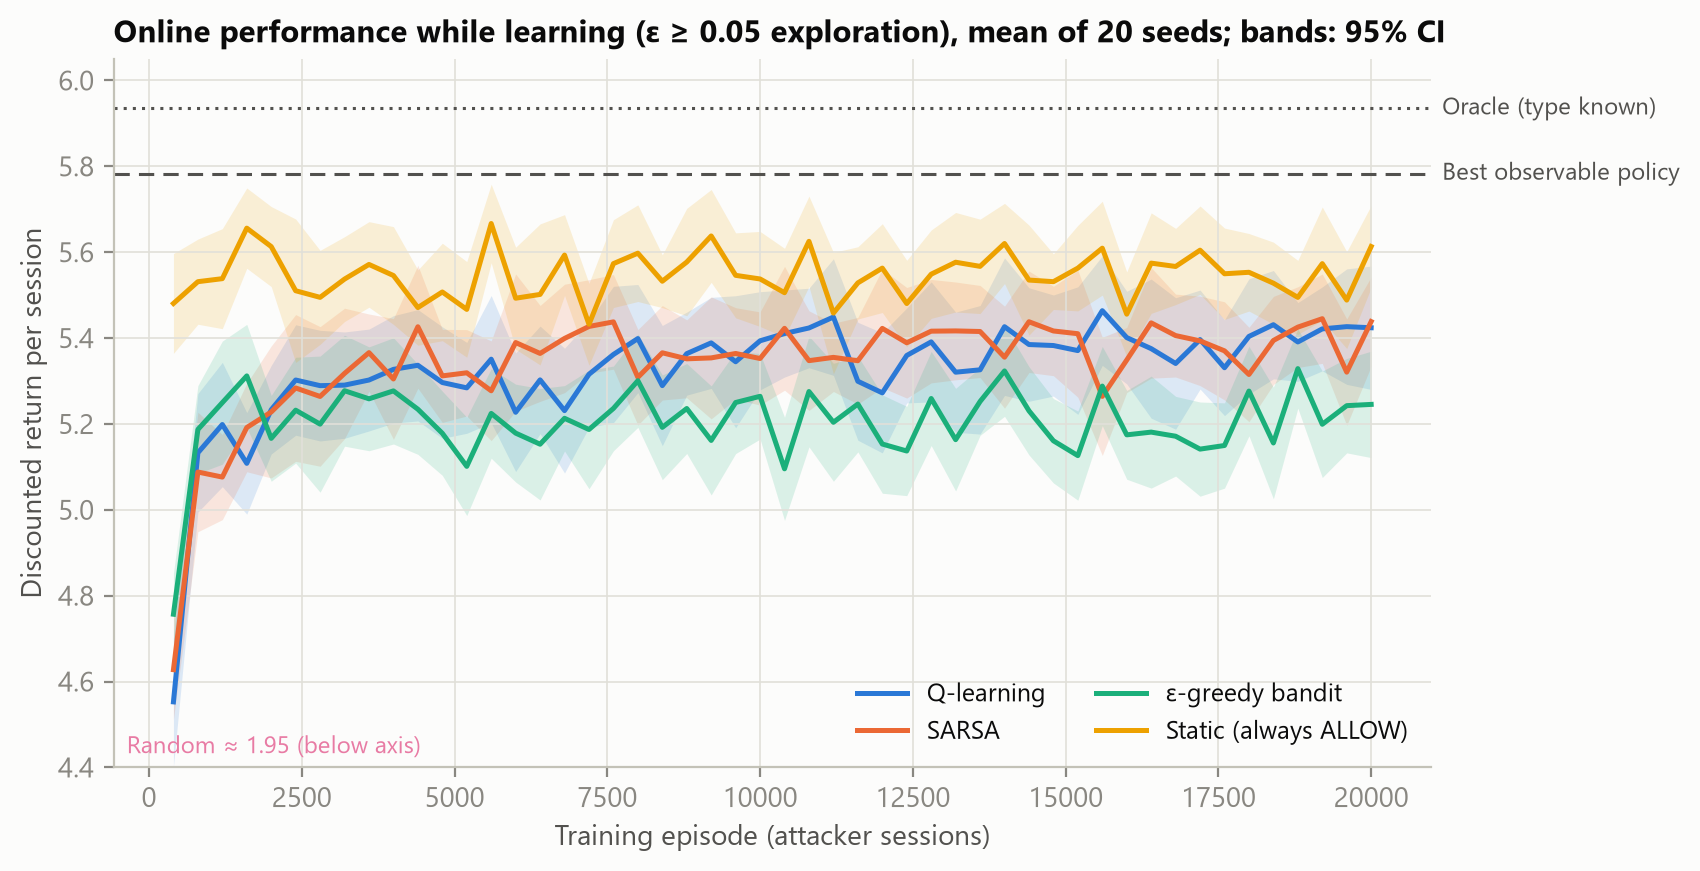
\includegraphics[width=\textwidth]{fig_learning_curves.png}
\caption{Online return during learning (block means of 400 episodes; bands are 95\% CIs over seeds).}
\label{fig:curves}
\end{figure}

Online performance includes exploration: with $\varepsilon \ge 0.05$, about one action in
twenty is random, and some of those are session-ending \act{block}s. During learning, all three
learners therefore stay \emph{below} the static honeypot (about 5.42 against 5.55 at the end),
even though the greedy policies they have learned are better than static. The exploration needed
to keep learning costs about as much as adaptation gains. In deployment, $\varepsilon$ should
therefore decay towards zero once the policy has settled. A GLIE schedule does this, as does
serving the greedy policy while learning off-policy from logged sessions.

\section{Step Size: a Negative Result Explained by Theory}

The first run used the constant step size $\alpha = 0.1$ from the original design. The learned
policies were \emph{worse} than the static honeypot: $5.343 \pm 0.154$ after 5{,}000 episodes,
better than static in only 2 of 10 seeds. The diagnosis follows Section~\ref{sec:learning}. With
constant $\alpha$, the noise in each estimate stays at about $0.23\sigma$. In the most visited
states, such as \code{recon|early}, the true differences between actions are of the same size,
because bots barely react to the response. The greedy choice is therefore decided by noise, and
half of the seeds chose a non-\act{allow} action there.

\begin{table}[H]
\centering
\begin{tabular}{@{}lcc@{}}
\toprule
\textbf{Step size} & \textbf{5{,}000 episodes} & \textbf{20{,}000 episodes} \\
\midrule
constant $\alpha = 0.1$ & $5.343 \pm 0.154$ \;(2/10) & $5.479 \pm 0.150$ \;(4/10) \\
$\alpha_n = n^{-0.6}$ & $5.662 \pm 0.080$ \;(9/10) & $5.618 \pm 0.138$ \;(7/10) \\
$\alpha_n = n^{-0.7}$ (main) & $5.608 \pm 0.155$ \;(8/10) & $\mathbf{5.710 \pm 0.043}$ \;(10/10) \\
$\alpha_n = n^{-0.85}$ & $5.610 \pm 0.092$ \;(7/10) & $5.676 \pm 0.067$ \;(8/10) \\
$\alpha_n = 1/n$ & $5.513 \pm 0.087$ \;(4/10) & $5.611 \pm 0.083$ \;(6/10) \\
\bottomrule
\end{tabular}
\caption{Step-size ablation (Q-learning, 10 seeds each). In parentheses: number of seeds whose final policy beats static (5.542).}
\label{tab:ablation}
\end{table}

\begin{figure}[H]
\centering
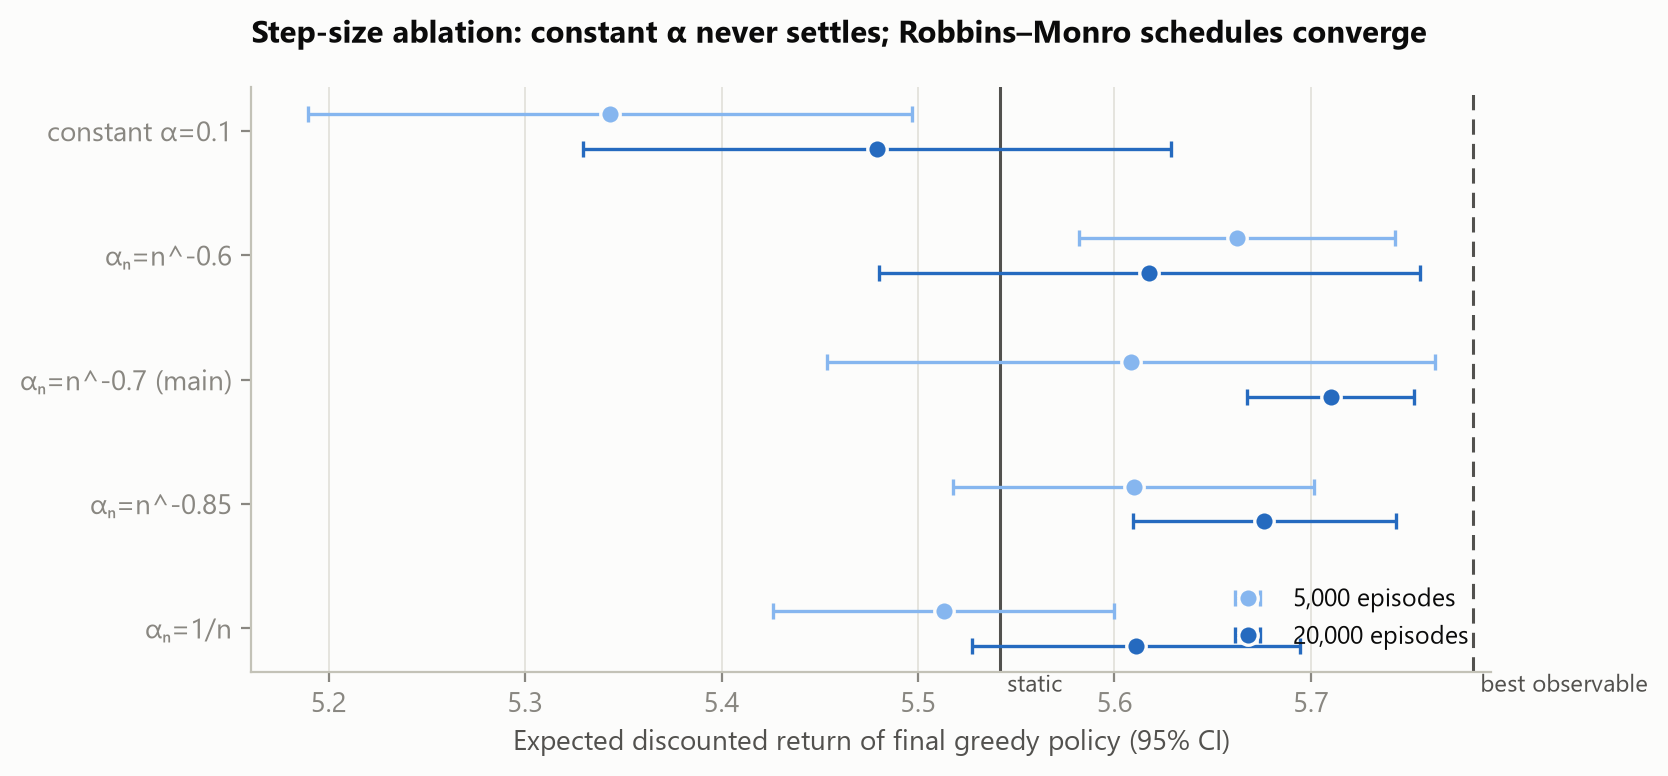
\includegraphics[width=0.92\textwidth]{fig_ablation_step_size.png}
\caption{Step-size ablation.}
\label{fig:ablation}
\end{figure}

The Robbins--Monro schedules all beat static. Among them, $1/n$ is the weakest. This agrees
with Even-Dar and Mansour~\cite{evendar2003rates}: with $1/n$, the early bootstrapped targets,
which are wrong, keep too much weight for too long. The differences among
$\omega \in \{0.6, 0.7, 0.85\}$ are not significant with 10 seeds. The robust conclusion is that
the step size must decay, and must decay more slowly than $1/n$.

\section{A Residual Bias}

In 95\% of runs Q-learning chooses \act{block} in \code{cleanup|late}, where the best observable
policy keeps \act{allow}. A diagnostic on fresh seeds found that the learned $Q(\act{allow})$
there is $1.18$ against a true $2.04$, while $Q(\act{block})$ is exact ($2.00$ against $2.00$).
Late states are rarely visited, so the values that \act{allow} bootstraps from are still near
their initial levels. \act{block}'s target is terminal and does not bootstrap. Once \act{block}
is greedy, \act{allow} receives only half as many updates (109 against 199), so the underestimate
persists. The cost is 0.0017 in return (0.03\%). Optimistic initial values or double
Q-learning~\cite{vanhasselt2010double} are standard remedies and are left as future work rather
than tuned on the reported seeds.

\section{RQ2: Sensitivity to Attackers and Objective}

\begin{table}[H]
\centering
\begin{tabular}{@{}llcccc@{}}
\toprule
\textbf{Mix} & \textbf{Objective} & \textbf{Static} & \textbf{Q-learning} & \textbf{Best obs.} & \textbf{Oracle} \\
\midrule
balanced & intel & 5.542 & $5.736 \pm 0.012$ & 5.783 & 5.935 \\
bot-heavy & intel & 5.133 & $5.159 \pm 0.039$ & 5.222 & 5.281 \\
human-heavy & intel & 6.273 & $6.600 \pm 0.060$ & 6.740 & 6.953 \\
balanced & attrition & 5.542 & $5.659 \pm 0.076$ & 5.783 & 5.937 \\
bot-heavy & attrition & 5.133 & $5.135 \pm 0.038$ & 5.222 & 5.282 \\
human-heavy & attrition & 6.273 & $6.634 \pm 0.055$ & 6.740 & 6.957 \\
\bottomrule
\end{tabular}
\caption{Sensitivity analysis (10 seeds per scenario). The attrition objective rewards attacker time consumed ($w_c = -0.05$).}
\label{tab:sens}
\end{table}

\begin{figure}[H]
\centering
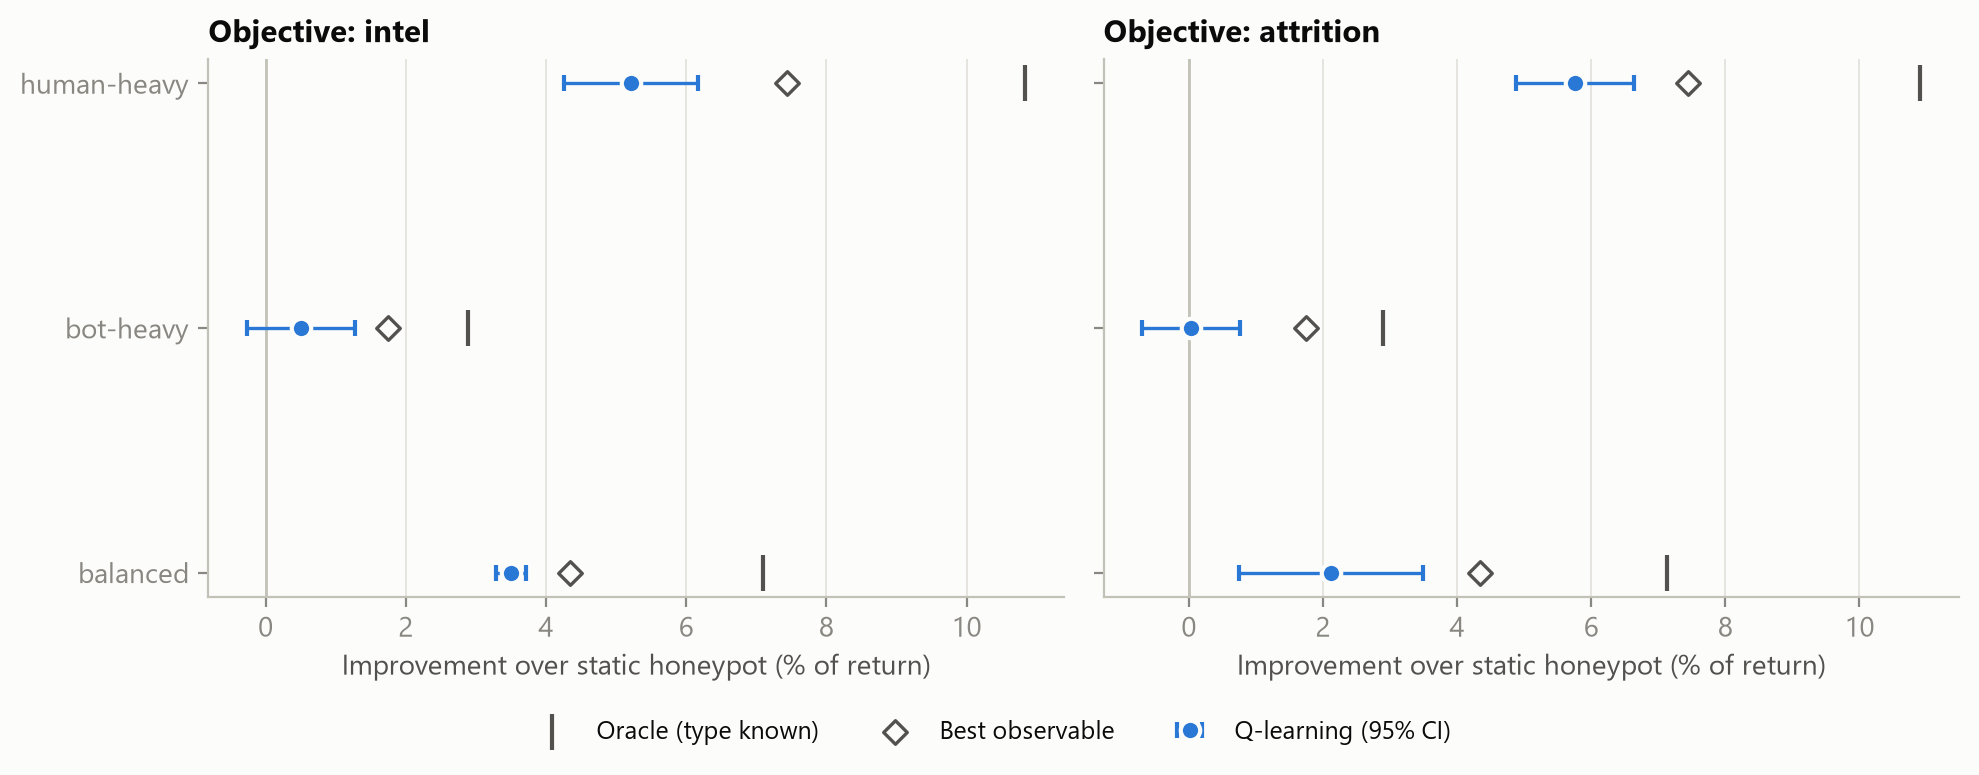
\includegraphics[width=\textwidth]{fig_sensitivity.png}
\caption{Improvement over the static honeypot by population and objective.}
\label{fig:sens}
\end{figure}

\begin{itemize}
  \item \textbf{Adaptation pays in proportion to how adaptive the attackers are.} The gain over
    static is $+0.5\%$ against bot-heavy traffic (not significant), $+3.5\%$ against the balanced
    mix and $+5.2\%$ against human-heavy traffic. Against scripted bots, a static honeypot is
    already near-optimal.
  \item \textbf{The learned structure is stable.} \act{fake} on credential access appears in every
    scenario. With many bots, the best policy also uses \act{fake} on file browsing. Under the
    attrition objective it uses \act{delay} on late cleanup, slowing down sessions that are
    about to end at no cost in intelligence.
  \item \textbf{\act{tarpit} is never chosen}, even when wasting attacker time is rewarded. Under
    this model, the sessions it would end are worth more than the time it would waste.
\end{itemize}

\section{Threats to Validity}

\begin{enumerate}
  \item \textbf{Model dependence.} Effect sizes depend on the assumed reaction multipliers. The
    qualitative conclusions hold in all six scenarios: static is near-optimal against bots,
    \act{fake} on credential access is the robust deviation, and the step size must decay.
    Fitting the model to captured sessions (Section~\ref{sec:fit}) is the way to tighten them.
  \item \textbf{Abstraction.} The simulator generates command categories, not command strings,
    so misclassification of real input is not modelled.
  \item \textbf{Stationarity.} Real attacker populations drift; the experiments use a fixed mixture.
  \item \textbf{Reward design.} Conclusions are also reported in reward-independent units
    (commands and intelligence per session).
  \item \textbf{Benchmark optimality.} The best observable policy is a strong local optimum of an
    NP-hard problem, not a proven optimum.
\end{enumerate}
